\documentclass[12]{article}
\usepackage[margin = 1in]{geometry}
\usepackage{amsmath}
\usepackage{listings}
\usepackage{graphicx}
\graphicspath{C:\Users\Abe\Documents\CEIRA Research\Large B approx}
\begin{document}

\title{Stability of Critical Points}
\author{Abraham Teklu}
\date{}
\maketitle
To look at the stability of the critical points of a linear, autonomous differential equation we used two methods. The first is to look at the phase plane of our two variables $V$ and $P$, here we relate them to population of two coexisting species. The second is to make a Jacobian matrix and find the eigenvalues. The equation that describes them is the following:
\begin{equation}
\frac{dP}{dt} = P\left(1-P-\frac{AV}{P+C}\right)
\end{equation} 
\begin{equation}
\frac{dV}{dt} = BV(1-\frac{V}{P})
\end{equation}
These two equation describe the growth rate of the two populations with respect to time and each other. When these two equations equal zero is when they are in equilibrium (have constant population); that is what the critical point describes. There are two critical points, when $(V,P) = (0,1)$ and $(V,P) = (P_c,P_c)$. The $P_c$ we are looking is positive real value to describe at what population  for both species can they coexist. The first solution is not interesting because it requires one species to be extinct.
$$\frac{dP}{dt} = P\left(1-P-\frac{AV}{P+C}\right) = 0~~~~~~~
\frac{P(1-P)(P+C)-AP^2}{P+C} = 0$$ 
We set $V = P$ because that is where the critical point is, and now we can simply solve for the numerator using the quadratic formula; $\gamma = A + C$.

$$P_c = \frac{1-\gamma}{2} + \frac{\sqrt{(1-\gamma)^2 + 4C}}{2}$$

These critical points can be seen as nodes on the phase plane. The node at which the species coexist is stable spiral, and the other node is an unstable saddle. This can be easily seen on the Phase Plane of V \& P shown below. To confirm what kind of nodes the two critical points we found the Jacobian matrix of the differential equations and then found their eigenvalues. Depending on the eigenvalues we can determine the type of node. The Jacobian matrix of two differential equations can be described as the following:
$$\frac{dP}{dt} = P\left(1-P-\frac{AV}{P+C}\right) = f$$ 
$$\frac{dV}{dt} = BV(1-\frac{V}{P}) = g$$

\begin{Large}
$$J = \begin{bmatrix}
\frac{\partial f}{\partial P} & \frac{\partial f}{\partial V}\\
\frac{\partial g}{\partial P} & \frac{\partial g}{\partial V}
\end{bmatrix}
$$
\end{Large}

\begin{equation}\tag*{}
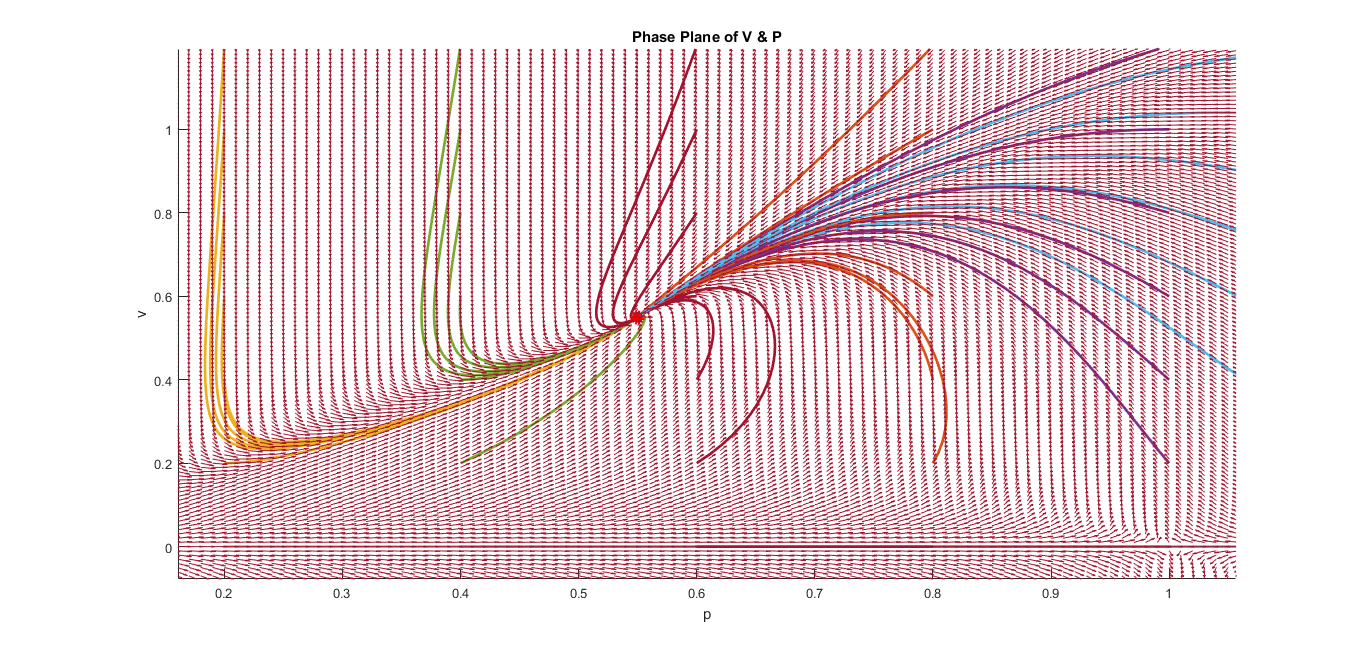
\includegraphics[scale=0.5]{LayredPhasePlaneandTrajectoryA0531818B2C01}
\end{equation}
\begin{small}
The figure above is has conditions A,B,C set to 0.531818,2,0.1 respectively. Also we are showing values of V that are less than zero simply to make it easier to see the node at (1,0); it does not have physical meaning.
\end{small}
\\
\\
\\
The jacobian matrix for these differential equations is:
\begin{Large}
$$J = \begin{bmatrix}
1-2P-\frac{AV}{P+C} + \frac{APV}{(P+C)^2} & \frac{-AP}{P+C}\\
\frac{BV^2}{P^2} & B - \frac{2BV}{P}
\end{bmatrix}
$$
\end{Large}
The eigenvalues for the coexistence critical point is:
$$\lambda_1 = -1.0846 + 0.2491i ~~~~~~~~~~~ \lambda_2 = -1.0846 - 0.2491i$$
The eigenvalues for the nonexistence critical point is:
$$\lambda_1 = 2 ~~~~~~~~~~~ \lambda_2 = -1$$
These eigenvalues confirm the conclusions we came to about the nodes. However, to understand these critical points we must know what happens for all parameters of A,B, and C. The first parameter we will look at is B. In equation (2) above B is a parameter for the change in population of the predator. If we do the following it is more understandable how B effects the critical point.
\begin{equation}
\frac{1}{B}\frac{dV}{dt} = V\left(1-\frac{V}{P}\right)
\end{equation}
This says at the coexistence critical point for $\frac{dV}{dt}\approx 0$, and so we can reduce our system of equations to a single equation B has to be sufficiently large. If we then ask what is the limit of B, as it approaches zero, for this simplification to be correct we come up with some interesting solutions. Most simply we can look at the difference in the critical points while keeping A and C constant.\\
\\
Graphic Figures[Here]
Graphic Description[Here]
\\
We can also calculate the relative error of these critical points and plot them as a function of B.
\begin{equation}\tag{p1}
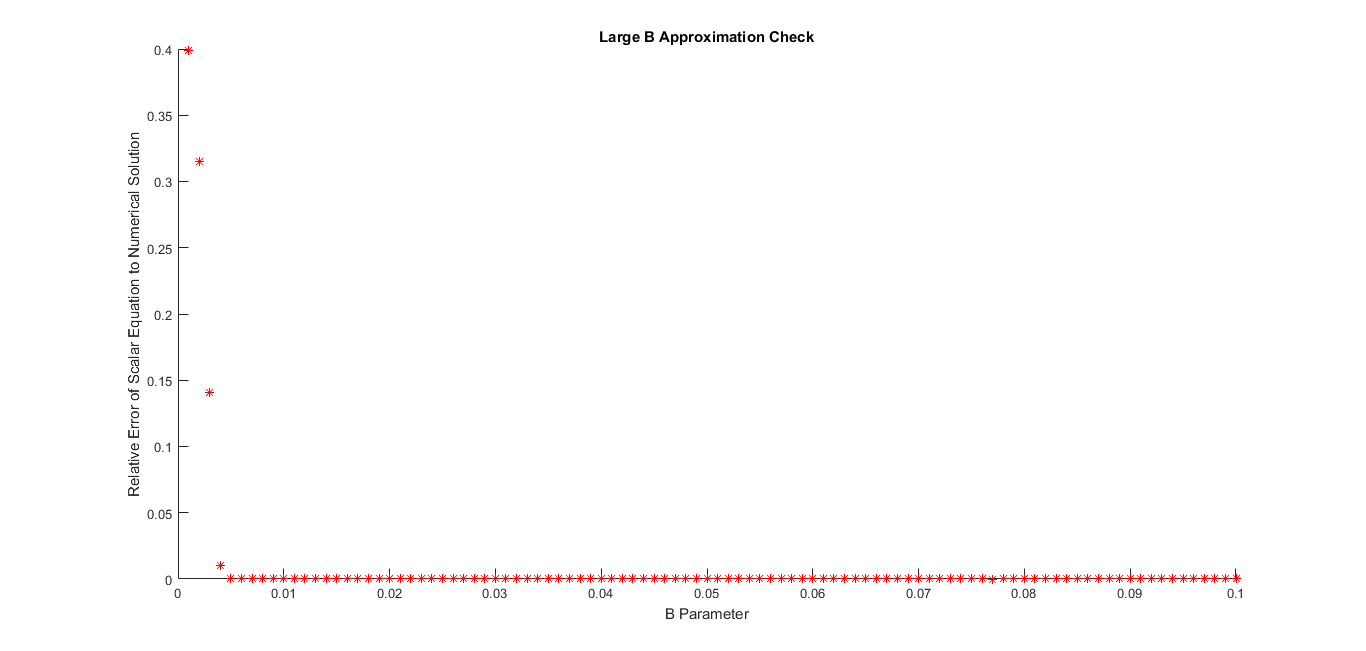
\includegraphics[scale=0.4]{RelativeErrofBPlot(sharp)}
\end{equation}
\begin{equation}\tag{p2}
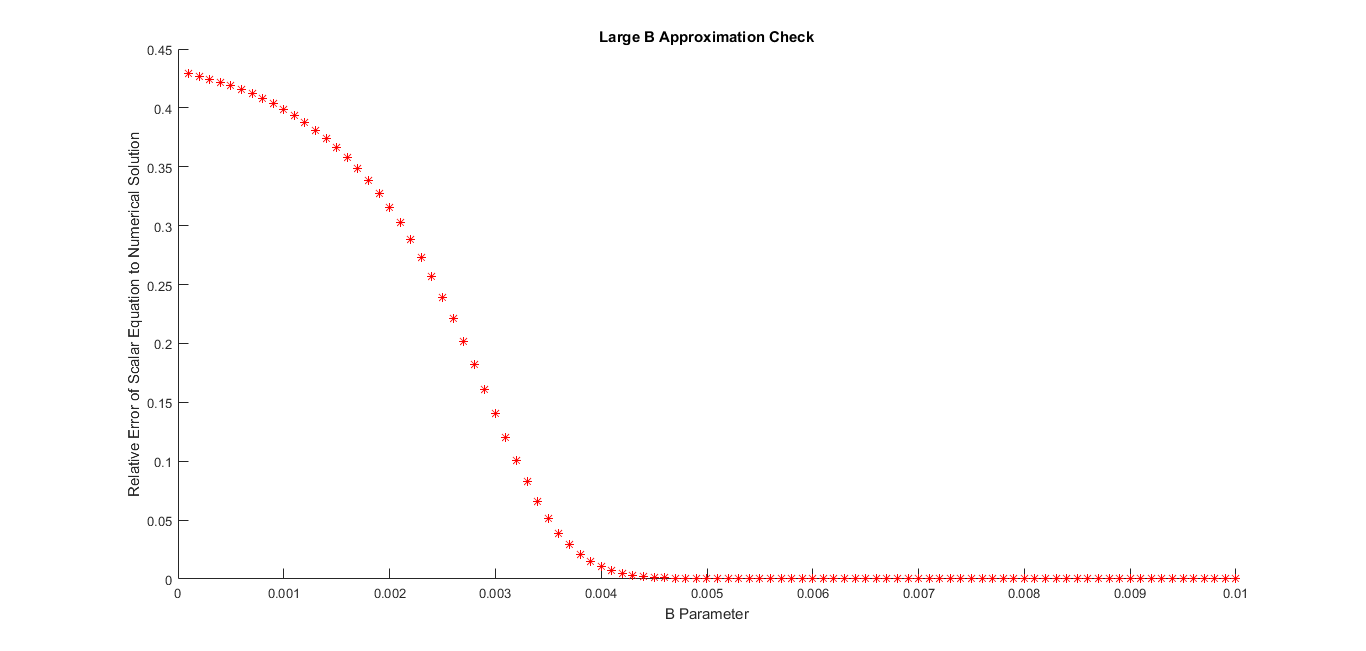
\includegraphics[scale=0.4]{RelativeErrofBPlot(smooth)}
\end{equation}
\begin{equation}\tag{p3}
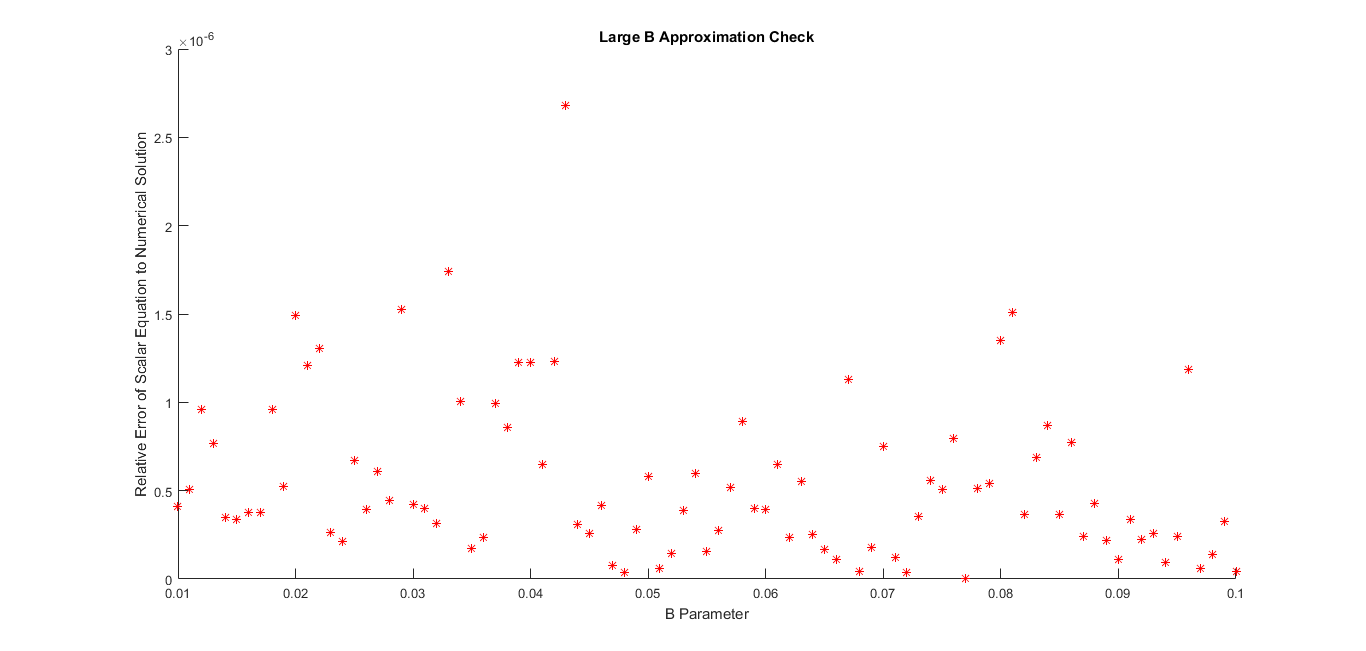
\includegraphics[scale=0.4]{RelativeErrofBPlot(rumble)}
\end{equation}

Plot one, or p1, is showing a the relative error of the critical critical point is huge for B values close to zero, but quickly becomes very small. Since the relative error is almost zero for B > 0.01 p2 was made to take a closer look at decline of the relative error. p2 shows that around B = 0.004 the relative error is less than 1\% and that the simplification of two differential equations to one differential equation is valid. p3 is a plot of what is occurring on the flat portion of p1; it shows that the relative error is not completely controlled by the trend of larger B gives smaller relative error.



\end{document}